% $Header: /projects/VU-SAGA/Papers/saga_engine_2006/generaldesign.tex,v 1.18 2006/10/11 02:55:39 gallen Exp $

The implementation level requirements of the SAGA reference
implementation as described in the previous section directly
motivate a number of design objectives. Our most important objective was to 
design a state-of-the-art Grid application framework satisfying the majority 
of user-needs while remaining as flexible as possible. 

This flexibility and extensibility of the implementation, 
 is then central to the design, and  dominates
the overall architecture of the library (see figure~\ref{fig:archi}).  As
a summary: only components known to be stable, such as the SAGA
``look\,\&\,feel'' and the SAGA utility classes, are statically included
in the library -- all other aspects of the API implementation, such as
the core SAGA classes and the middleware compile time and run time
bindings, are designed to be components which can be added and
selected separately.

\begin{figure}[!ht]
 \begin{center}
  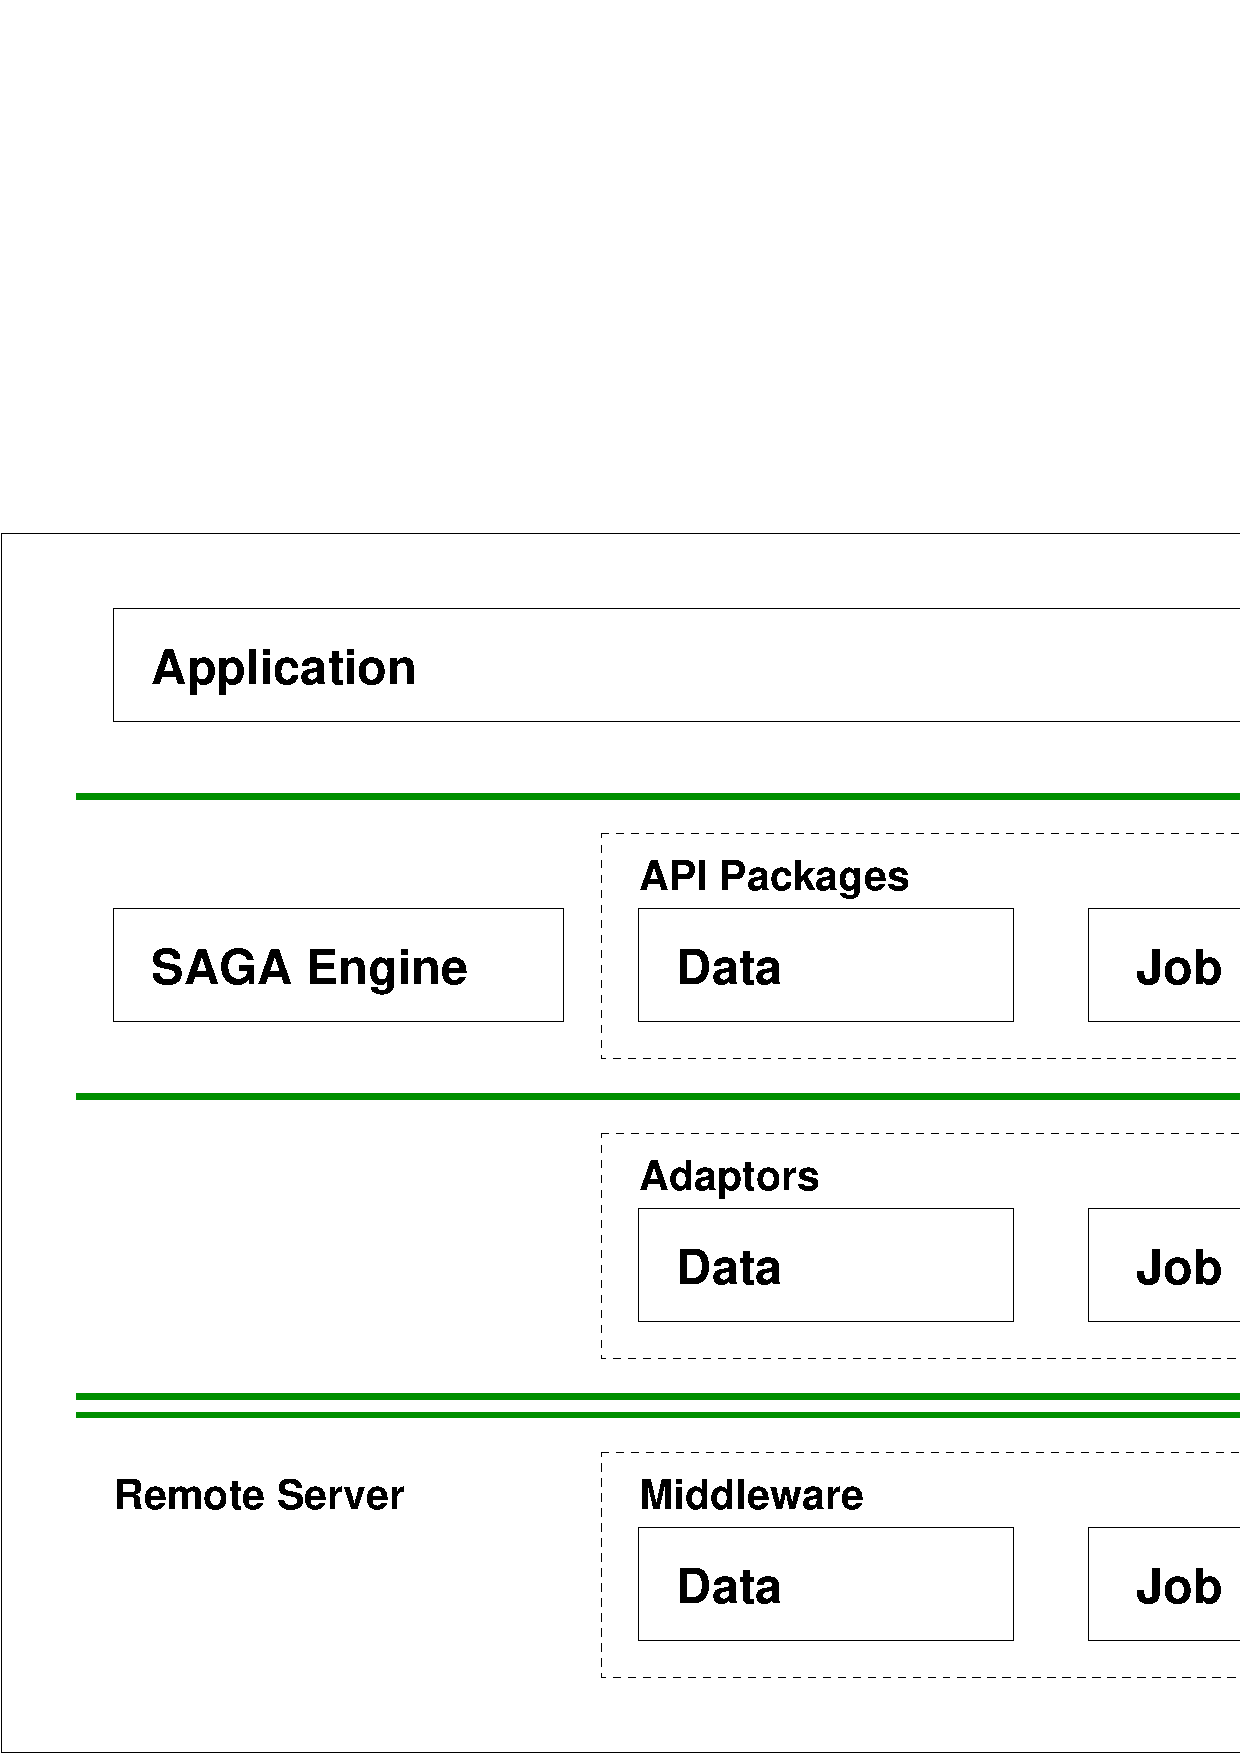
\includegraphics[width=0.47\textwidth]{images/saga_architecture}
  \up
  \caption{\label{fig:archi}
    Architecture: A lightweight engine dispatches SAGA 
    calls to dynamically loaded middleware adaptors.  See text for
    details.}
 \end{center}
\end{figure}

\up
\subsection{Design Objectives}

  Although the Simple API for Grid Applications is, by definition
  \I{simple} for application developers,  this doesn't imply that the
  implementation itself has to be simple. We made a major effort to
  build	as much logic and functionality as possible into the SAGA
  library core, providing all the needed common functionality. This	enables
  the user to extend it with minimal effort. On the other hand, the
  library \I{is} designed to be easy to build, use, and deploy. 
	
	A major design
	objective was to maximize decoupling of different components
	of the developed library to provide  as much \I{flexibility}, 
	\I{adaptability} and \I{modularity} as possible.

	As the SAGA implementation is expected to be used on different platforms
	and operating systems we strive for maximal implementation \I{portability}. 

  The API should be \I{extensible} with minimal effort: ideally,
  adding a new API class is orthogonal to all other properties of the
  implementation.


\subsection{The Overall Architecture}

	To meet these goals we decided to decouple the library components
	in three completely orthogonal dimensions -- 
	the user of the library may use and combine these freely and 
	develop additional suitable components usable in tight integration with 
	the provided modules.

\subsubsection{Horizontal Extensibility -- API Packages}
\label{ssec:apipackages}

  Our implementation uses the grouping of sets of API functions as defined
  by the SAGA specification to define \I{API  packages}.	 
  Current packages are: file management, job management,
  remote procedure calls, replica management, and data streaming. 
  These modules depend only on the SAGA engine, the user is free to
  use and link only those actually needed by the application,
  minimizing the memory footprint.
  It is straightforward to add new packages (as the SAGA specification 
  is expected to evolve) since all common
  operations needed inside these packages (such as adaptor loading and
  selection, or method call routing) are imported from the SAGA
  engine.  The creation of new packages is essentially reduced to:
  (1) add the API package files, and declare the classes, (2) reflect the 
  SAGA object hierarchy (see section~\ref{ssec:pimpl}), and (3) add class 
  methods.

  The declaration and implementation of the API methods is simplified by
  macros, which essentially correspond directly to the methods
  SIDL specification (see section~\ref{ssec:macros}).  We are
  considering (partly) automating new package generation, by parsing
  the SIDL specification and generating the class stubs and class
  method specifications.  
  Additionally, this approach will also allow us to generate
  other SAGA language bindings from the SIDL specification, such as
  for C and FORTRAN.
  
\subsubsection{Vertical Extensibility -- Middleware Bindings}

  A layered architecture (see figure~\ref{fig:archi}) allows us to
  vertically decouple the SAGA API from the used middleware. Separate
  adaptors, either loaded at runtime, or pre-bound at link time,
  dispatch the various API function calls to the appropriate
  middleware. 
	These adaptors implement a well
  defined \I{Capability Provider Interface} (CPI) and expose that to the
  top layer of the library, making it possible to switch adaptors
  at runtime, and hence to switch between different (even concurrent)
  middleware services providing the requested functionality. 
  
  The top library layer dispatches the API function calls to the
  corresponding CPI function.  It additionally contains the \I{SAGA
  engine} module, which implements: (1) the core SAGA objects such 
  as session, context, task or task\_container -- these objects are 
  responsible for the SAGA look\,\&\,feel, and are needed by all API 
  packages, and (2) the common functions to load and select matching 
  adaptors, to perform generic call routing from API functions to the 
  selected adaptor, to provide necessary fall back implementations 
  for the synchronous and asynchronous variants of the API functions 
  (if these are not supported by the selected adaptor).
	
	The dynamic nature of this layered architecture enables easy future 
	extensions by adding new adaptors, coping with emerging grid standards 
	and new grid middleware.
	

\subsubsection{Extensibility for Optimization and Features} 

  Many features of the engine module are implemented by intercepting,
  analyzing, managing, and rerouting function calls between the API packages,
  (where they are issued) and the adaptors (where they are executed
  and forwarded to the middleware).  To generalize this management
  layer, a PIMPL~\cite{pimpl} (Private IMPLementation) 
  idiom was chosen, and is rigorously
  used throughout the SAGA implementation.  This PIMPL layering allows
  for a number of additional properties to be transparently
  implemented, and experimen\-ted with, without any change in
  the API packages or adaptor layers.  These features
  include: generic call routing, task monitoring and optimization, 
  security management, late binding, fallback on adaptor invocation errors,
  and latency hiding mechanisms.
	The decoupling of these features from the API and 
  the adaptors succeeds, essentially, because these properties 
  affect only the IMPL side of the PIMPL layers.  

  The engine module is thus fully generic, and loosely coupled to
  both the API and adaptor layers.  Any engine feature, all
  optimizations, latency hiding techniques, monitoring features etc.
  are implemented in generically, and are orthogonal to
  the API and adaptor extensions.  
